\documentclass[a4paper,10pt]{report}
\usepackage{geometry} % change page margins/layout
%\usepackage[ngerman]{babel} % document Germanisation
\usepackage[utf8]{inputenc} % German umlauts
\usepackage[T1]{fontenc} % accented language characters
\usepackage{bm} % better bold symbols
\usepackage{graphicx} % better image handling
\graphicspath{ {images/} }
\usepackage{wrapfig} % text wrap around images
\usepackage{subfig,caption} % subfigures and caption width
\usepackage[section]{placeins} % float barriers
\usepackage{booktabs} % better looking tables
\usepackage{makecell} % multi-rows in table cells
\usepackage[shortlabels]{enumitem} % better lists
\usepackage{amsmath,mathtools,amssymb} % math typesetting/symbols
\usepackage{nicefrac} % in-line looking fractions
\usepackage[version=4]{mhchem} % chemical elements
\usepackage[locale = US, 
			separate-uncertainty,
			exponent-product = \cdot,
			output-product = \cdot,
			per-mode=reciprocal]{siunitx} % easy uncertainties
\usepackage[hyphens]{url} % allows for URL breaks
\usepackage[colorlinks=true,linkcolor=black,
			urlcolor=blue,citecolor=black]{hyperref} % URL links
\usepackage[english]{cleveref} % better referencing
\usepackage{titlesec} % title section formatting
\titleformat{\chapter}{\bfseries\LARGE}{\thechapter~}{0em}{}
\usepackage[autostyle]{csquotes} % better quotes

% DARK-MODE on PDF reader
\usepackage{xcolor}
\pagecolor[HTML]{1f1f1f} % dark color
\color[HTML]{c7c7c7} % light color

\setcounter{tocdepth}{3}
%------------------------------------------------------------------


\begin{document}


\title{
	\vspace{2cm}
	{\LARGE Electric Vehicles in Energy Communities:}
	{\Large Investigating the Distribution Grid Hosting Capacity} \\[2cm]
	{\large Albert Ludwig University of Freiburg}
}
\author{
	\Large Daniil Aktanka
}
\date{
	\normalsize \today
}
\maketitle
\thispagestyle{empty}


\pagenumbering{roman}
\chapter*{Abstract}
\addcontentsline{toc}{chapter}{Abstract}


\tableofcontents
\cleardoublepage
\pagenumbering{arabic}


\chapter{Introduction}
\chapter{Literature Review}
Good intro into EV situation and market: \cite{Das2020}

Really good method, but I can't math: \cite{Gruosso2019}

\chapter{Goal and Method}
\section{Approach}\label{section_approach}
To reiterate, the goal of this thesis was to investigate the distribution grid hosting capacity of electric vehicles and the effect the involvement of energy communities can have on it. Over the span of roughly two months, the method presented in this paper went through many iterations in terms of functionality as well as network application. The original testing models were performed on a simple test network with generic coordinates and arbitrary values (see \cref{test_network}). These tests were done in order to get a feel for the chosen software tools and to better understand the potential real world application and its scope of work.

\FloatBarrier
\begin{figure}[htpb]
		\centering
		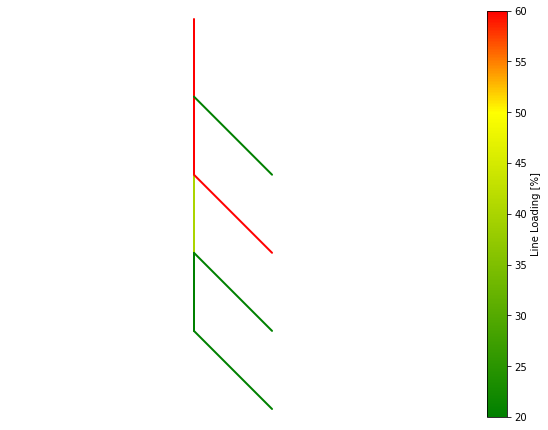
\includegraphics[width=0.46\linewidth]{test_network}
		\caption{An example test power flow calculation plot with line loading results. Here, one static generator is active out of four.}
		\label{test_network}
	\end{figure}
\FloatBarrier

Early on, it was decided to incorporate real-world data as a basis of the simulation. Arguably the best (at the time of writing) data platform for this application is Open Power System Data---more specifically, the contributed household data package. It contains measured time series data for various households and businesses relevant for low-voltage power system modeling. In terms of geographical scope, it incorporates data from 11 households in Konstanz, southern Germany, as part of the CoSSMic project for the optimization of energy systems in smart cities. The gathered data is quite expansive, spanning a time range of over 4 years with a resolution of up to 1 minute measurements, even tracking single-device consumption. Cumulative energy measurements accounted for data gaps in communication problems and "all data gaps are either interpolated linearly, or filled with data of prior days" \cite{OpenPowerSystemData}, though no further detail is provided in this regard. Overall, this was the perfect fit for my simulation aimed at a standard European low-voltage grid.

Using and incorporating the Open Power System Data household dataset proved to be quite a challenge on its own. Details regarding final data analysis are described in \cref{section_data_processing}. Once the data was processed and loaded into the network for further computations, the question became how to formulate and subsequently evaluate simulation scenarios. Hereby, the number of variables to take into account can practically be expanded far beyond the scope of the paper. For instance, an alternative tool considered for the simulation data was the LoadProfileGenerator (LPG), which is a highly-customizable tool for modeling residential energy consumption. LPG performs complete behavior simulation of a household residents in order to generate load curves. To that extent, it would have been possible to take said curves and implement them into our network case, while investigating individual households' behaviors across a community of like-minded, cooperative individuals. However, this was deemed far too comprehensive given the time constraints, but also not as potentially insightful.

Additionally, in order to make best use of the historical data, it was decided to perform time series iteration power flows. In a sense, this provides a similar advantage to LPG functionality by mimicking random human behavior over time, only with no unnecessary explanations behind it. The main idea became to sample a random historical load profile per household and to consider when/how an EV charger could optimally function in time. While this may be a relatively simple question to answer for a single household---given the residents' preferences and habits, it's merely a load optimization problem---the main issue lies with multiple parties involved. In turn, those parties are connected on a network in different ways, bringing topology into account. Thus, time and space both dictate the conditions for a given network.

Eventually, the rather abstract test network got superseded by the benchmark European Low Voltage Test Feeder (from hereon: test feeder) (see \cref{EU_LV_test_feeder}). Three scenarios were chosen for evaluation: critical case, random charging, semi-coordinated charging. The critical case is used for hosting capacity evaluation of our simulation for a single time point, whereas the two other scenarios demonstrate time-dependent charging behavior models. Detailed explanation for this approach is given in \cref{section_network_application}.

\FloatBarrier
\begin{figure}[htpb]
	\centering
	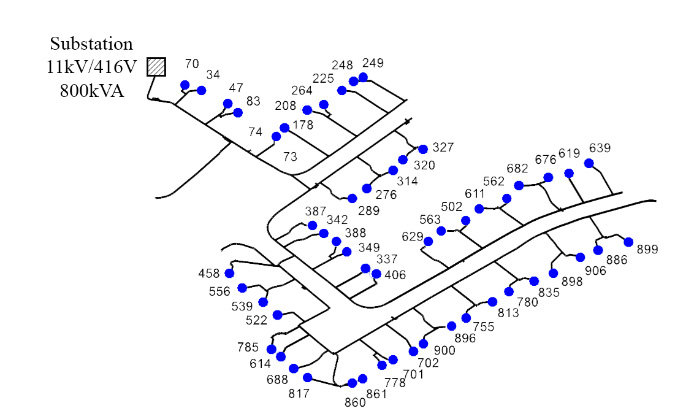
\includegraphics[width=0.7\linewidth]{EU_LV_test_feeder}
	\caption{European Low Voltage Test Feeder network illustration. The blue dots are the active busses, representing households \cite{Nousdilis2017}.}
	\label{EU_LV_test_feeder}
\end{figure}
\FloatBarrier

The next section will describe the functionality of custom python classes. For more details, consult the source code on GitHub at: \url{https://github.com/akthonka/EV_energy_comm} .

\newpage
\section{Data processing}\label{section_data_processing}
Given the scope of the project, the idea was to create a system flexible enough for iterative data manipulation and ideally one that would support multiple network types. The project was written entirely in python due to language simplicity as well as availability of advanced modules. Data handling was done using the \texttt{pandas} module, whereas the network simulation was performed using the \texttt{pandapower} module.

For the sake of clarity, most of the code was split between a python class file and jupyter notebooks. For early testing and code prototyping, jupyter notebooks are sufficient but they quickly lose readability as the code complexity grows. The general methodology was therefore to write core functions in jupyter to then integrate them into an external python class file. The resultant python class file consists of two classes: one for handling data processing and another for operations based on the \texttt{pandapower} module. Common input settings (for instance, the time window) are saved as class variables, such that only the most top-level functions are called in jupyter.

\subsection{DataAction class}
The following information describes the code of the python class responsible for core data processing. While the general methodology is applicable to any dataset, these functions are tailored specifically to the household dataset and will be described as such. Additionally, the functions mentioned here target the test feeder network as our simulation case but can be adapted for any network, with several caveats mentioned later.

The paragraphs serve to summarize the operation of one or more functions based on their application.

\paragraph{Data import and segmenting:} The raw dataset is imported as a dataframe without additional options. Dropping the rest, we keep only 3 columns: \texttt{DE\_KN\_residential1\_grid\_import}, \texttt{DE\_KN\_residential2\_grid\_import} and \texttt{utc\_timestamp}. Since we will be performing conditional time-based operations, we set the timestamp column as index for ease of use. While it is possible to front-load a lot of data processing functions at this step---such as parsing datetimes---it is not recommended due to unnecessary computation time. A better approach is to segment the data for piece-wise processing and function testing, whereby it would be possible to iterate computations over the entire dataset in the future. Therefore, we split the imported dataframe (of a little over a million data points) into a list of smaller dataframes (each 10000 data points long, with residual last dataframe being a bit smaller).

\paragraph{Datetime parsing function:} This function converts a segment of the imported data into a specific, time-indexed dataframe. First, we parse datetime index, specifying the format as \texttt{"Year--Month--Day Hour:Minute:Second"}, after which we convert from UTC to Berlin time---the local time of the recorded dataset. While it is possible to import data with local time column \texttt{cet\_cest\_timestamp} without the need of conversion, it is not recommended for \texttt{pandas 1.4.3} since that will cause errors in datetime operations based on my experience. Second, we take the difference between consecutive rows. This is done in order to obtain minute-wise energy changes, since the household dataset only tracks cumulative energy values. If we use the \texttt{pandas.diff()} function, we must also drop the resulting first row, since it's a NaN row.

\paragraph{Night profile functions:} This set of functions is fundamental for the simulation, as they are used to create a load profile for a single household. First, we must select a random dataframe segment with either of the two historical load profiles and parse it for datetime. The segment contains data on several days/nights, the dates of which we must identify. Then, for a random date, we must get the starting and ending datetimes for dataframe slicing. Knowing the starting time of our window---in our case, 18:00:00---we need to create a datetime object for the chosen date, given the starting time. From said datetime (for example, \texttt{2015-08-16 18:00:00}) we add one day to the date and update the time with our morning value (getting \texttt{2015-08-17 06:00:00}). With these two datetimes, we can now slice the selected dataframe to obtain the required single house overnight load profile.

\paragraph{Create loads and static generators:} This function creates the dataframes used for timeseries iteration---from hereon referred to as night dataframes. These hold the inputs for the network values, for both the loads as well as the static generators (sgens). Depending on the timeseries controller, it is important to create the night dataframes in a very specific way: the names and the indices of the network components will dictate the conventions. Unless you are writing your own controller, refer to your documentation for more details.

To create the night dataframes, first get a random night profile. This contains all the necessary time steps in the index, which is what we need; the load values can be set to zero. Then, generate a list of appropriate load names and form a dataframe using the time index. For the case of the test feeder network, the resulting night dataframes are 721 rows $\times$ 55 columns (minutes $\times$ number of profiles). Repeat for both loads and sgens night dataframes. It is recommended to save these as class variables, since we will be referencing them throughout the entire simulation, as well as for troubleshooting purposes. Finally, we convert our night loads to MW via a simple conversion factor multiplication.

\paragraph{Random static generators:} These functions fill the night sgen dataframe at random times with a select sgen value. It's recommended to first reset the night dataframe by setting all sgen values to zero, otherwise location slicing may not overwrite the value. Getting a random set of starting and ending datetimes follows the same principle as described for night profile functions. It's important to keep track of zero-based indexing when calling random values from range. Additionally, in case of \texttt{pandapower}, the sgen sign needs to be set as negative in order to act as a separate static load that is an EV charger.

\paragraph{Energy community static generators:} These functions fill the night sgen dataframe consequently and cyclically (see \cref{section_network_application} for motivation). This method consists of two parts. In the first part, the starting times for sgens are determined. The allowed time values are bound by the time window, and are dependent on the time step (charging time). To compute the list of starting charging times, begin with the evening time value and add the time step iteratively for the number of sgens present. In our case, we have 55 sgens and a time window of 12 hours; for a charging time of 1 hour, that would result in 12 starting charging times. If we only had 7 sgens in the same time conditions, we would have 7 starting charging times, etc. The next part concerns the starting time sgen cycle.

For best practice, set all night sgen values to zero before writing new ones. The following step was done using \texttt{cycle} function from the \texttt{itertools} module in python. Beginning with the evening start time, write the sgen charging value for the first generator, for the entire charging duration minus the last minute. The next minute, when the first generator is no longer active, fill the charging time window for the second generator, minus the last minute. Repeat the process until the last unique starting charging time is reached, after which the next starting charging time will loop back to the beginning of the list. Repeat this process for all given sgens. The looping time values can be handled with an extra class placeholder-variable for starting times instead of an entire additional look-up table.


\subsection{NetworkCalculation class}
The following information describes the code of the python class generally responsible for functions related to the \texttt{pandapower} module. In particular, its main purpose is perform timeseries iteration on a specific network. An additional function to calculate the hosting capacity is also contained here. The NetworkCalculation class is meant to be used directly in conjunction with the DataAction class and contains several direct references to it.

\paragraph{Network preparation and controllers:} In order to perform the timeseries iteration we first need to prepare our network. In the case of our chosen simulation---test feeder network---this involves some additional steps (see next section). First, create the network, including the loads and sgens. It's recommended to stick to a consistent naming convention for loads and sgens across the network properties and the external night dataframes, in order to avoid unnecessary problems when configuring the controller in the next step.

The controller is a function whose purpose is to update the network values iteratively from a look-up table. The methodology will depend on your software of choice, but in our case we will be using the \texttt{pandapower} controllers made specifically for timeseries module. \Cref{timeseries_module_diag} shows a general overview of the built-in module.

\FloatBarrier
\begin{figure}[htpb]
		\centering
		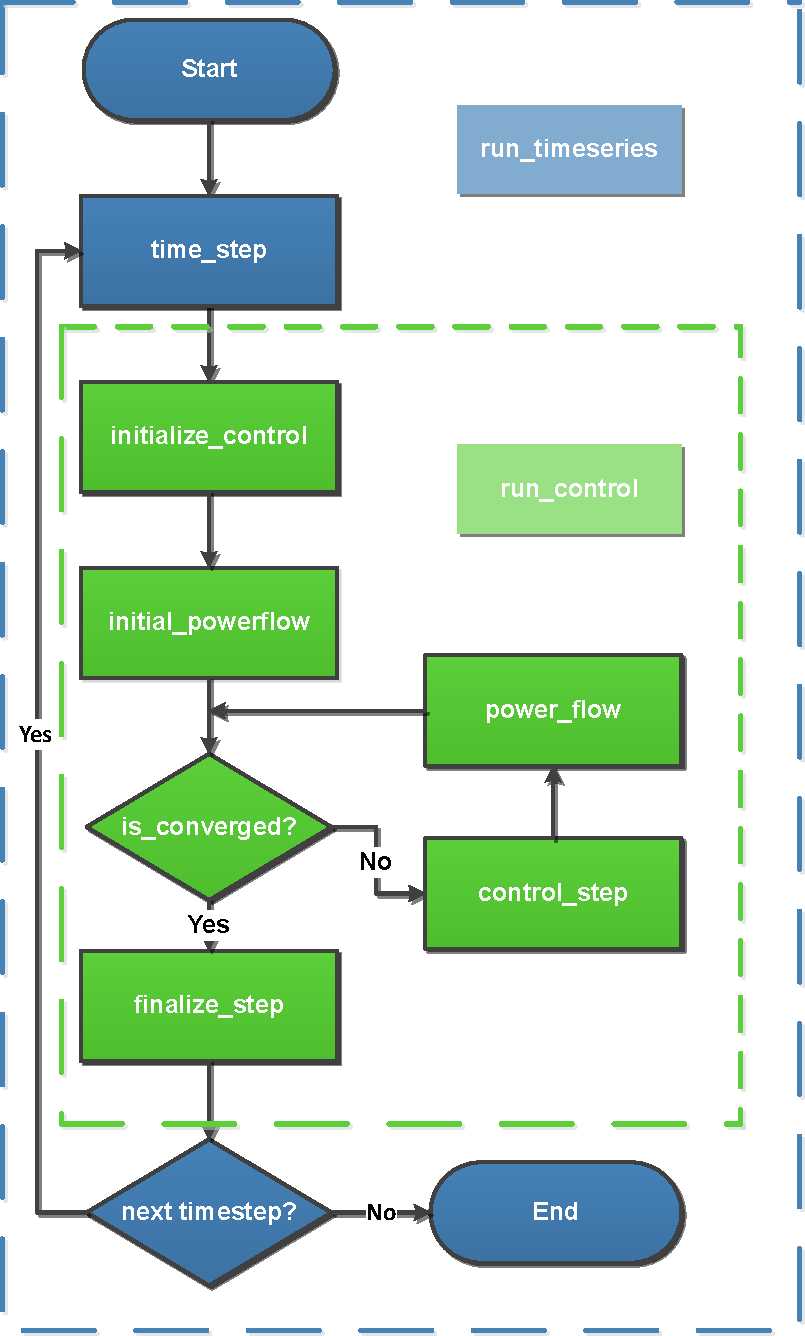
\includegraphics[width=0.35\linewidth]{timeseries_module_diag.pdf}
		\caption{The diagram shows the time series loop of the time series module. The basic functionality is compute the power flow for each time step using the given values---such as sgens or loads. Step-wise convergence will depend on several factors, such as the network parameters (i.e. load magnitudes) as well as the algorithm used for solving the power flow problem. For more module details, see the \texttt{pandapower}  \href{https://pandapower.readthedocs.io/en/v2.10.1/timeseries/timeseries_loop.html}{wiki}.}
		\label{timeseries_module_diag}
	\end{figure}
\FloatBarrier

For our simulation, we will need 2 constant controllers for loads and sgens. Hereby, the correspondent data sources are the night dataframes that were defined in the DataAction class. Lastly, the timeseries iteration needs to be given a defined number of time steps, which in our case will be given by the index length of (either) night dataframe. With this information, the power flow can be computed iteratively based on tabular variable inputs. However, this will yield no useful results on its own, which is why we need to additionally define an output writer.

\paragraph{Time iteration and output:} An output writer is a function with a simple job of recording computed information, in an desired format, for each timeseries step. In our case, we will again be using the output writer function supplied with the \texttt{pandapower} timeseries module and outputting into an Excel file for the sake of convenience and troubleshooting. However, we aim to continue data processing in \texttt{pandas}, so we define another import function for said Excel results file. The imported dataframe can now provide relevant statistics and metrics. For our evaluation, the one of the key computations is the all-time minimum load value across all busses (see \cref{section_network_application} for more details).

\paragraph{Hosting capacity evaluation:} Hosting capacity was computed iteratively for a network in a single point in time. All pre-loaded network settings (even from the timeseries iteration) stay the same, except for the sgen columns---those need to be set to zero at first. Do not confuse the night sgen dataframe with the network sgen column; for a single point in time, only the network-defined sgens are taken into the calculation.

Iteration was performed over the list of sgen indices using a \texttt{for} loop. The list is scrambled prior iteration in order to mimic uncoordinated charging patterns. An additional variable for storing the hosting capacity count is created. For each cycle of the loop, the following metric variables are computed by running a power flow calculation: minimum bus voltage magnitude (per unit) and maximum line loading percent. The next step is conditional. If the metric variables don't exceed preset limits, add an sgen value and increase the hosting capacity count by one. The loop proceeds onto the next cycle and computes the new power flow state of the network. Checking the metric variables again, if (at some point) the preset limits are exceeded, then we need to undo the effects of the last cycle. As such, the hosting capacity count is reduced by one and the last filled sgen is reset to zero. This breaks the loop. The function then computes one final power flow computation to obtain for an output plot and prints the maximum hosting capacity result.

\section{Network application}\label{section_network_application}
This section builds upon the fundamental operating principles of the two classes introduced in \cref{section_data_processing}. It aims to explain the usage of the python class file in order to obtain the three scenarios for the test feeder.

%Assumptions:\\
%Treating three-phase network as single phase\\
%Network asymmetric loads set to zero\\
%Adjusting the historical load magnitude\\
%1 hr window because...\\

The network used in the simulation is an alteration of the standard test feeder. The original network itself is 3-phase, which would require a different power flow model---in case of \texttt{pandapower}, that would be handled by \texttt{pandapower.pf.runpp\_3ph.runpp\_3ph()}. However, given the right circumstances, it is possible to treat a 3-phase network as single-phase; namely, if we assume that all network loads are balanced. This assumption is plausible and corresponds to most real-world households, to the extent that some power modeling software (such as BLANK) don't even include a separate 3-phase computation option for this reason. With this assumption, all loads and sgens were defined and handled as single-phase in our simulation.

Furthermore, the standard test feeder was (in most cases) not able to support direct application of the household load profiles. During timeseries iteration, the console encounters a singular-matrix error, indicating that the Jacobian cannot be solved for this power flow. In practical terms, this meant that the network was overloading at some point in time. Indeed this point in time was almost certainly converging to the average evening peak load time for this dataset. From past applications of data analysis, with data spanning over 500 days, the average maximum load time (across both households 1 and 2) was calculated to be \texttt{19:19:00} (in a time bracket of \texttt{18:00:00--06:00:00}). The solution was to scale the historical load curves. The resultant network busses, with no sgens active, fall in an acceptable voltage magnitude per unit range between 1.03 and 1.05. FOR WHATEVER REASON, GOTTA EXPLAIN

Another assumption that was made concerns the charging times---these were meant to stay constant in length. MOST CHARGERS ON THE MARKET... MOST AVERAGE EVS... BLAH BLAH, 1 HOUR CHARGING TIME GOTTA EXPLAIN

With these assumptions and adjustments to the test feeder, the following 3 case scenarios were identified and analyzed.

\subsection{Critical case scenario}
single point in time at peak load\\
compute max number of sgens active, random location\\

\subsection{Random time scenario}
night time window\\
random sgen locations\\

\subsection{Energy community scenario}
night time window\\
semi-ordered sgen locations\\
semi-coordinated charging\\


\chapter{Results and Discussion}
\section{Results}

\FloatBarrier
\begin{figure}[htpb]
		\centering
		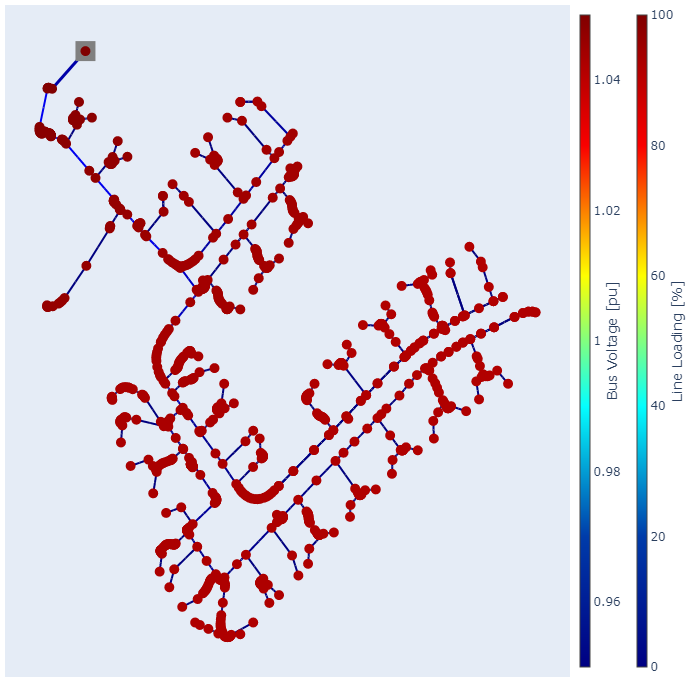
\includegraphics[width=0.9\linewidth]{EU_LV_host_critical}
		\caption{blahblah}
		\label{EU_LV_host_critical}
	\end{figure}
\FloatBarrier

\FloatBarrier
\begin{figure}[htpb]
	\centering
	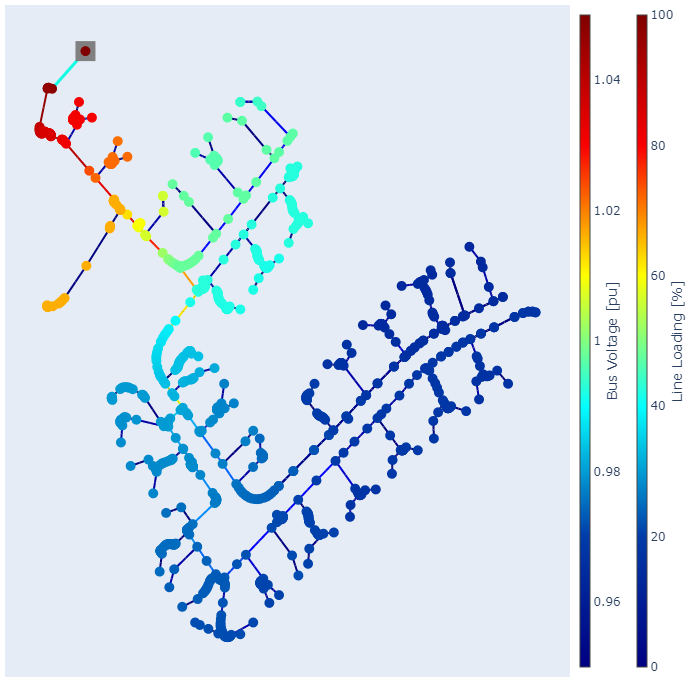
\includegraphics[width=0.9\linewidth]{EU_LV_host_capacity}
	\caption{blahblah}
	\label{EU_LV_host_capacity}
\end{figure}
\FloatBarrier



\section{Suggested improvements}


\chapter{Conclusion}
\bibliographystyle{IEEEtran} %displays URLs
\bibliography{bib_library}

\chapter*{Appendix}
\addcontentsline{toc}{chapter}{Appendix}


\end{document}

%------------------------------------------------------------------

%\FloatBarrier
%\begin{figure}[htpb]
%	\centering
%	\includegraphics[width=0.9\linewidth]{blah}
%	\caption{blah}
%	\label{blah}
%\end{figure}
%\FloatBarrier